% DGPO in piRL: group-meeting slides. Build: tectonic dgpo_pirl.tex
% Figures come from ../figures/make_figures.py (all numbers from ../README.md).
\documentclass[aspectratio=169,11pt]{beamer}
\usetheme{default}
\usecolortheme{default}
\setbeamertemplate{navigation symbols}{}
\setbeamertemplate{footline}[frame number]
\setbeamerfont{frametitle}{series=\bfseries}
\definecolor{ink}{HTML}{0B0B0B}
\definecolor{ink2}{HTML}{52514E}
\definecolor{dgpo}{HTML}{2A78D6}
\definecolor{prism}{HTML}{EB6834}
\definecolor{grpo}{HTML}{1BAF7A}
\setbeamercolor{frametitle}{fg=ink}
\setbeamercolor{title}{fg=ink}
\setbeamercolor{structure}{fg=dgpo}
\setbeamercolor{alerted text}{fg=prism}

\usepackage{booktabs}
\usepackage{graphicx}
\usepackage{amsmath,amssymb}
\usepackage{tabularx}
\usepackage{array}
\graphicspath{{../figures/}}
\newcolumntype{Y}{>{\raggedright\arraybackslash}X}
\newcommand{\pirl}{$\pi$RL}
\newcommand{\pizero}{$\pi_0$}
\newcommand{\pifive}{$\pi_{0.5}$}
\newcommand{\up}[1]{\textcolor{grpo}{\textbf{#1}}}
\newcommand{\snote}[1]{{\footnotesize\textcolor{ink2}{#1}}}

\title{DGPO inside \pirl}
\subtitle{Replacing Flow-SDE GRPO with Direct Group Preference Optimization\\for flow-based VLAs (\pifive)}
\author{Jiyong Kwon, Purdue University}
\date{September 2026}

\begin{document}

\begin{frame}
  \titlepage
\end{frame}

\begin{frame}{The question}
  \begin{itemize}
    \item Plan from the postdoc: pick an RL method (Flow-GRPO, DGPO, Prism-GRPO),
          put it into \pirl, and post-train \pizero\ / \pifive.
    \item \textbf{Idea 1 (Euclidean):} keep \pirl's model, environments, rollouts and reward;
          \textbf{replace only the Flow-GRPO update with DGPO} (arXiv:2510.08425).
    \item DGPO's claim: no stochastic policy needed, deterministic ODE rollouts,
          $\sim$20--30$\times$ faster than Flow-GRPO on image generation.
    \item Stage 2: swap the binary success reward for Prism-GRPO's
          $R = \text{success} + \lambda q$ (arXiv:2608.17423).
  \end{itemize}
  \vspace{0.6em}
  \textbf{Answer in one line:} in every setting we tested, \pirl's GRPO improves the policy
  more and faster than DGPO; Prism adds nothing measurable.
\end{frame}

%==================================================================
\section{Setup}
\begin{frame}{What is what: the components of a \pirl\ experiment}
  \small
  \begin{tabularx}{\linewidth}{@{}l Y Y Y@{}}
    \toprule
    Component & What it is & \pirl\ options & \textbf{Used here} \\
    \midrule
    Model (policy) & VLA that outputs actions & \pizero, \pifive & \textbf{\pifive} \\
    SFT data & demos used before RL & per benchmark (next slide) & RLinf's released SFT checkpoints \\
    Environment & simulator the policy acts in & LIBERO, ManiSkill, MetaWorld, CALVIN & all four \\
    Action & command sent to the robot each step & 4--7 dims (next slide) & benchmark default \\
    RL algorithm & update rule from rewards & PPO (main), GRPO & \textbf{GRPO, DGPO} \\
    Exploration noise & how the flow sampler is made stochastic & Flow-SDE, Flow-Noise & Flow-SDE; DGPO: ODE or SDE \\
    Reward & score of a trajectory & binary success & binary; \textbf{Prism} \\
    \bottomrule
  \end{tabularx}
\end{frame}

\begin{frame}{Benchmarks: environment, action, data, reward}
  \scriptsize
  \begin{tabularx}{\linewidth}{@{}l Y Y Y Y@{}}
    \toprule
    & LIBERO & ManiSkill & MetaWorld & CALVIN \\
    \midrule
    Robot & Franka Panda & WidowX (Bridge) & Sawyer & Franka Panda \\
    Tasks & 4 suites $\times$ 10 (Spatial, Object, Goal, Long) & 16 objects $\times$ 17 receptacles $\times$ 16 scenes & MT50: 50 tasks & chains of 5 subtasks; train ABC, eval D \\
    \textbf{Action} & 7-d: $\Delta$pos 3, $\Delta$rot (axis-angle) 3, gripper & 7-d: $\Delta$EEF pose 6, gripper & \textbf{4-d}: $\Delta$xyz 3, gripper & 7-d: $\Delta$pos 3, $\Delta$rot (Euler) 3, gripper \\
    \textbf{SFT data} & few-shot demos; 40 trajectories, one \pifive\ checkpoint for all suites & 16,384 MPLib motion-planning episodes & official set, 2,500 trajectories & CALVIN ABC play data ($\sim$24 h) \\
    Reward & success 1 / 0 & 1.0 success + 0.1 grasp & success 1 / 0 & subtask success \\
    Episode & 240 steps (Long 480) & 80 & 100 & 480 / subtask \\
    SFT (ours, noise-free) & 0.806 (Spatial), 0.274 (Long) & 0.447 & 0.461 & 0.136 \\
    \bottomrule
  \end{tabularx}
\end{frame}

\begin{frame}{\pirl's own variants and what we ran}
  \small
  \begin{columns}[T]
    \column{0.5\linewidth}
    \textbf{\pirl\ paper, Table 1 (PPO), success \%}\\[0.3em]
    \scriptsize
    \begin{tabular}{@{}llcccc@{}}
      \toprule
      & & LIBERO & MS & MW & CALVIN \\
      \midrule
      \pizero & SFT & 57.6 & 38.4 & 50.8 & 57.5 \\
      & Flow-SDE & 96.1 & 78.8 & 78.1 & 61.7 \\
      & Flow-Noise & 97.6 & 77.8 & 85.8 & 59.9 \\
      \midrule
      \pifive & SFT & 77.1 & 40.1 & 43.8 & 61.3 \\
      & Flow-SDE & 97.9 & 90.9 & 70.7 & 87.0 \\
      & Flow-Noise & 98.3 & 89.7 & 66.1 & 84.5 \\
      \bottomrule
    \end{tabular}\\[0.3em]
    \snote{GRPO is reported only on LIBERO (Table 4, \pifive\ avg.\ 91.5).}
    \column{0.46\linewidth}
    \textbf{Our runs (all \pifive, 12 h each)}\\[0.3em]
    \tiny
    \begin{tabular}{@{}lccccc@{}}
      \toprule
      & Sp. & Long & MW & MS & CV \\
      \midrule
      GRPO + Flow-SDE & \checkmark & \checkmark & \checkmark & \checkmark & \checkmark \\
      DGPO, ODE & \checkmark & \checkmark & & & \\
      DGPO + SDE & \checkmark & & \checkmark & \checkmark & \checkmark \\
      DGPO + SDE + Prism & \checkmark & & \checkmark & \checkmark & \checkmark \\
      DGPO, 1-step noise & & & \checkmark & \checkmark & \\
      \bottomrule
    \end{tabular}\\[0.4em]
    \snote{Our absolute numbers sit below the paper's: a 12 h budget is
    20--200 steps on 4$\times$H100, the paper trains longer on 8.}
  \end{columns}
\end{frame}

%==================================================================
\section{How to run it}
\begin{frame}{The training loop (RLinf), and where DGPO plugs in}
  \small
  \begin{enumerate}
    \item \textbf{Rollout:} env workers step the simulator; rollout workers sample action chunks
          from the flow policy. Groups of 8 envs share one reset state.
    \item \textbf{Reward \& advantage:} binary success per trajectory $\to$ GRPO-normalised
          $A_i$ within each group (or Prism's RLOO advantage).
    \item \textbf{Update (the only part we replace):}
      \begin{itemize}
        \item GRPO: clipped ratio of the Gaussian transition log-probs at one noised denoise step.
        \item DGPO: forward-noise the clean chunk $x_0$, $x_t=(1-t)x_0+t\epsilon$; score it with the
              DSM loss of the policy and of a frozen SFT reference; group-level sigmoid.
      \end{itemize}
    \item \textbf{Held-out eval:} noise-free (ODE) sampler, 512 episodes per checkpoint
          (CALVIN: 50--200), same config for every method.
  \end{enumerate}
\end{frame}

\begin{frame}[fragile]{Reproducing a run}
  \scriptsize
  \textbf{Code:} \texttt{\textasciitilde/pirl-dgpo/RLinf} (branch \texttt{dgpo}): \texttt{rlinf/algorithms/dgpo.py},
  \texttt{workers/actor/fsdp\_dgpo\_policy\_worker.py}, configs \texttt{*\_dgpo\_openpi\_pi05.yaml}, \texttt{*\_grpo\_openpi\_pi05.yaml}.
\tiny
\begin{verbatim}
# DGPO on MetaWorld (SDE 0.3 on every denoise step, 2 updates/rollout)
sbatch --export=ALL,CONFIG=metaworld_50_dgpo_openpi_pi05,\
  CKPT=$L/checkpoints/RLinf-Pi05-MetaWorld-SFT,EXTRA_PYTHONPATH=$L/envpkgs/metaworld \
  jobs/01_dgpo_libero_spatial.sbatch

# ...with GRPO's exact exploration noise (one random step, 0.5)
  ... +actor.model.openpi.nft_single_noise_step=True actor.model.openpi.noise_level=0.5

# ...with the Prism reward
  ... algorithm.filter_rewards=False +algorithm.dgpo_reward=prism +algorithm.prism_lambda=0.5

# GRPO control arm
sbatch --export=ALL,CONFIG=metaworld_50_grpo_openpi_pi05,... jobs/02_pirl_grpo_baseline.sbatch

# Held-out eval of any checkpoints (noise-free, 128 envs x 4 epochs)
sbatch --export=ALL,EVAL_CONFIG_DIR=...,EVAL_CONFIG=metaworld_50_dgpo_openpi_pi05_eval,... \
  jobs/03_eval_ckpts.sbatch sft /path/to/global_step_20/actor/model_state_dict/full_weights.pt
\end{verbatim}
  \snote{Configs are generated from \pirl's PPO configs by \texttt{jobs/make\_dgpo\_configs.py} /
  \texttt{make\_grpo\_configs.py}: only the algorithm, the sampler and the training env's reset change.}
\end{frame}

\begin{frame}{Cluster notes (Expanse, 4$\times$H100 per node)}
  \footnotesize
  \begin{itemize}
    \item One Python env (\texttt{rlinf\_venv}); MetaWorld and CALVIN deps are side-installed with
          \texttt{--target} and added through \texttt{EXTRA\_PYTHONPATH} (MetaWorld needs gymnasium 1.x,
          which would break LIBERO).
    \item ManiSkill's Vulkan renderer works only on some nodes (exp-19-15/16/17); others fail with
          \texttt{ErrorDeviceLost} at camera creation.
    \item CALVIN's EGL renderer SIGABRTs mid-rollout; we use pybullet's CPU renderer
          (\texttt{CALVIN\_USE\_EGL=0}).
    \item Every job gets its own Ray port block and temp dir (shared nodes); no \texttt{ray stop}.
    \item LIBERO eval on Long needs the robosuite horizon raised (\texttt{+env.eval.init\_params.horizon=3000}).
    \item Budget used: $\sim$1.5k of 10k H100-hours.
  \end{itemize}
\end{frame}

%==================================================================
\section{Method}
\begin{frame}{DGPO, and how it maps onto an MDP}
  \small
  DGPO (Eq.~17) for a group $\mathcal G$ sharing a condition $c$:
  \[
    \mathcal L = -\log\sigma\!\Big(-\beta \textstyle\sum_{x\in\mathcal G} A(x)\,
      \big[\mathcal L^{\theta}_{\text{dsm}}(x) - \mathcal L^{\text{ref}}_{\text{dsm}}(x)\big]\Big),
    \qquad \textstyle\sum_{\mathcal G^+}|A| = \sum_{\mathcal G^-}|A| \Rightarrow Z(c)\text{ cancels.}
  \]
  \begin{itemize}
    \item Images: sample $=$ one image, $c=$ the prompt.
    \item \pirl: every chunk sees a different observation, so no two chunks share $c$.
          What a group shares is the \textbf{reset state}.
    \item $\Rightarrow$ \textbf{sample $=$ trajectory}: $\log\frac{\pi_\theta(\tau)}{\pi_{\text{ref}}(\tau)}
          = \sum_k \log\frac{\pi_\theta(a_k|o_k)}{\pi_{\text{ref}}(a_k|o_k)}$ (dynamics cancel);
          each chunk term $\to$ its DSM difference, averaged over the trajectory's valid chunks.
    \item A principled trajectory-level extension, not the paper's theorem
          (the closed form needs deterministic dynamics, which MuJoCo has).
  \end{itemize}
\end{frame}

\begin{frame}{Implementation and verification}
  \small
  \begin{itemize}
    \item The sigmoid spans all chunks of all trajectories in a group ($\sim$8$\times$48 forward passes),
          so the loss cannot be micro-batched, but its gradient can:
          \[ \partial\mathcal L_g/\partial \mathcal L^{\theta}_{ik} \propto \sigma(-z_g)\,A_i
             \;\Rightarrow\; \text{no-grad pass for } z_g,\ \text{then backprop } \textstyle\sum \sigma(-z_g)A_i\,\mathcal L^\theta_{ik}. \]
    \item Unit tests (15): surrogate gradient $=$ autograd of the exact objective; $Z$ cancels;
          masking; length balance.
    \item \textbf{Matches the official code:} our gradient equals the gradient of
          \texttt{compute\_group\_dgpo\_loss\_allreduce} (read from Luo-Yihong/DGPO) for
          $\beta\in\{1,10^2,10^4\}$.
    \item Two bugs found and fixed on the way: summed (not length-normalised) chunk terms made long
          failures dominate and collapsed training to 0\%; metric averaging over idle ranks.
  \end{itemize}
\end{frame}

%==================================================================
\section{Before vs after exploration noise}
\begin{frame}{Before noise: the paper's setting (ODE rollouts) makes the policy worse}
  \centering
  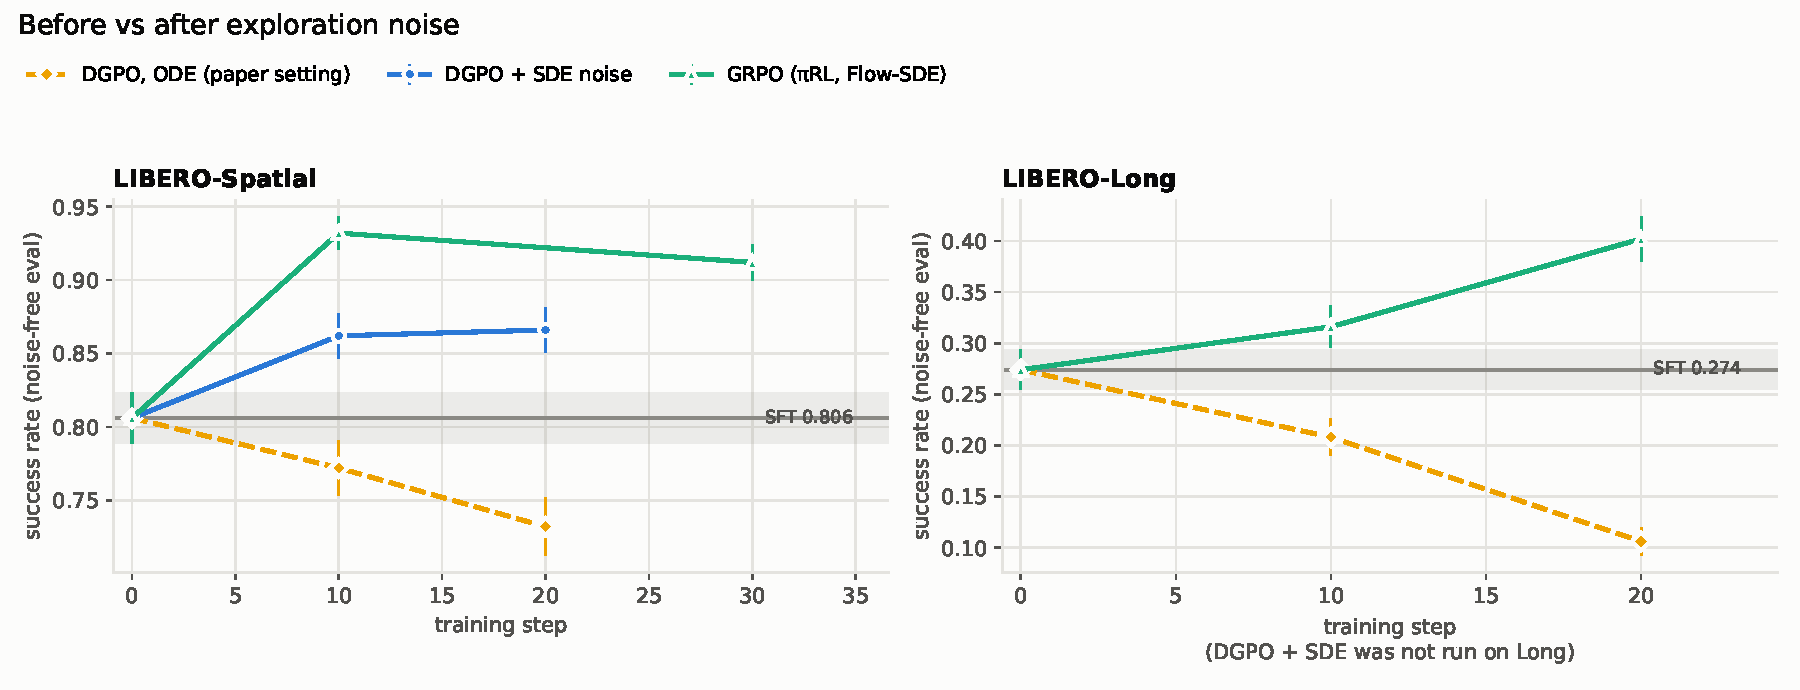
\includegraphics[width=0.95\linewidth]{fig5_noise_before_after.pdf}\\
  \snote{Noise-free held-out success, 512 episodes, $\pm$1 s.e. Step 0 $=$ SFT.
  ODE DGPO falls below SFT on both LIBERO suites and keeps falling.}
\end{frame}

\begin{frame}{Why the noise is needed}
  \small
  \begin{itemize}
    \item With ODE rollouts the 8 trajectories of a group differ only in their initial noise.
          The SFT policy is already strong ($\sim$0.88 on Spatial), so they behave almost alike:
          only $\sim$40\% of groups have mixed outcomes.
    \item Pushing the likelihood of a failed trajectory down also pushes down the many chunks it
          shares with successful ones.
    \item A step-matched SFT control (lr $=0$) showed the early ``drops'' were partly reset-state
          difficulty, so every run is compared on held-out evals, never on training success.
    \item Adding SDE noise (DGPO's own ``w/ SDE'' variant) raises mixed groups to $\sim$90\%,
          and DGPO starts to learn.
  \end{itemize}
\end{frame}

\begin{frame}{What it took to make DGPO learn (LIBERO-Spatial, step 10)}
  \centering
  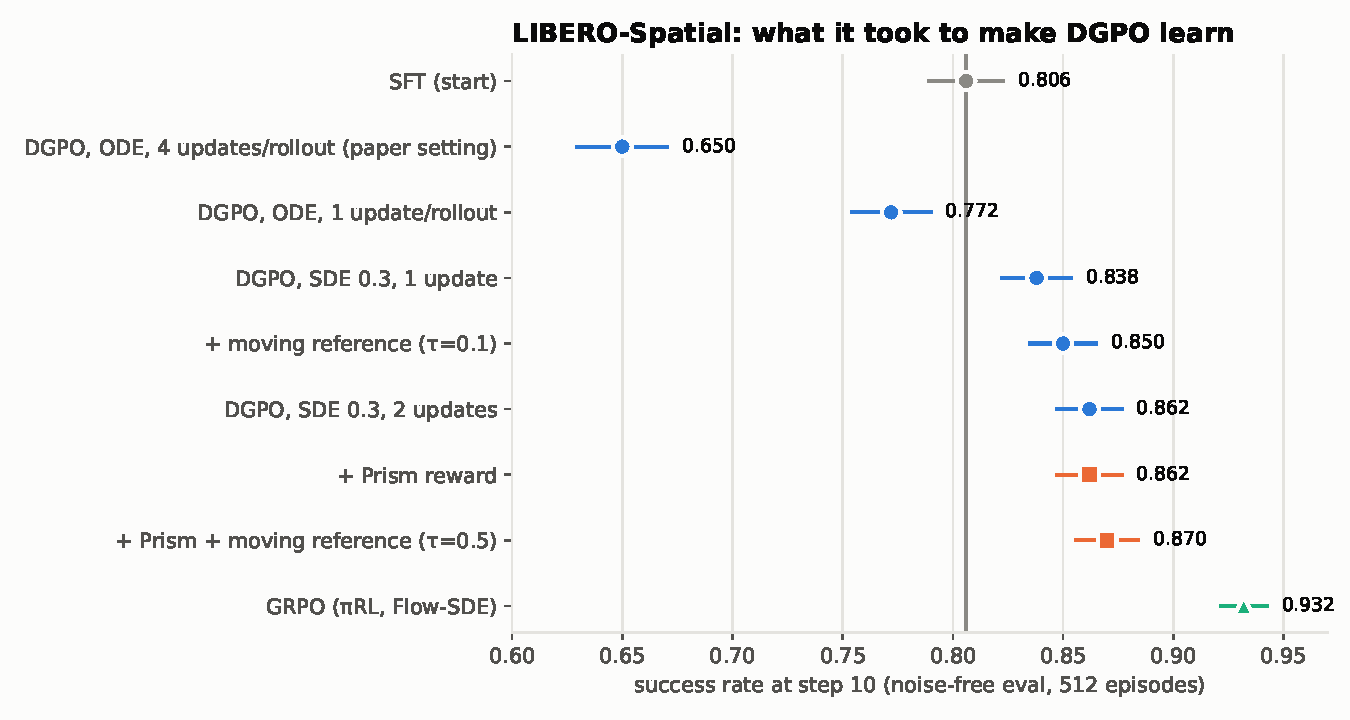
\includegraphics[width=0.78\linewidth]{fig3_libero_ablation.pdf}
\end{frame}

%==================================================================
\section{Results after adding noise}
\begin{frame}{After noise: best improvement over SFT, all benchmarks}
  \centering
  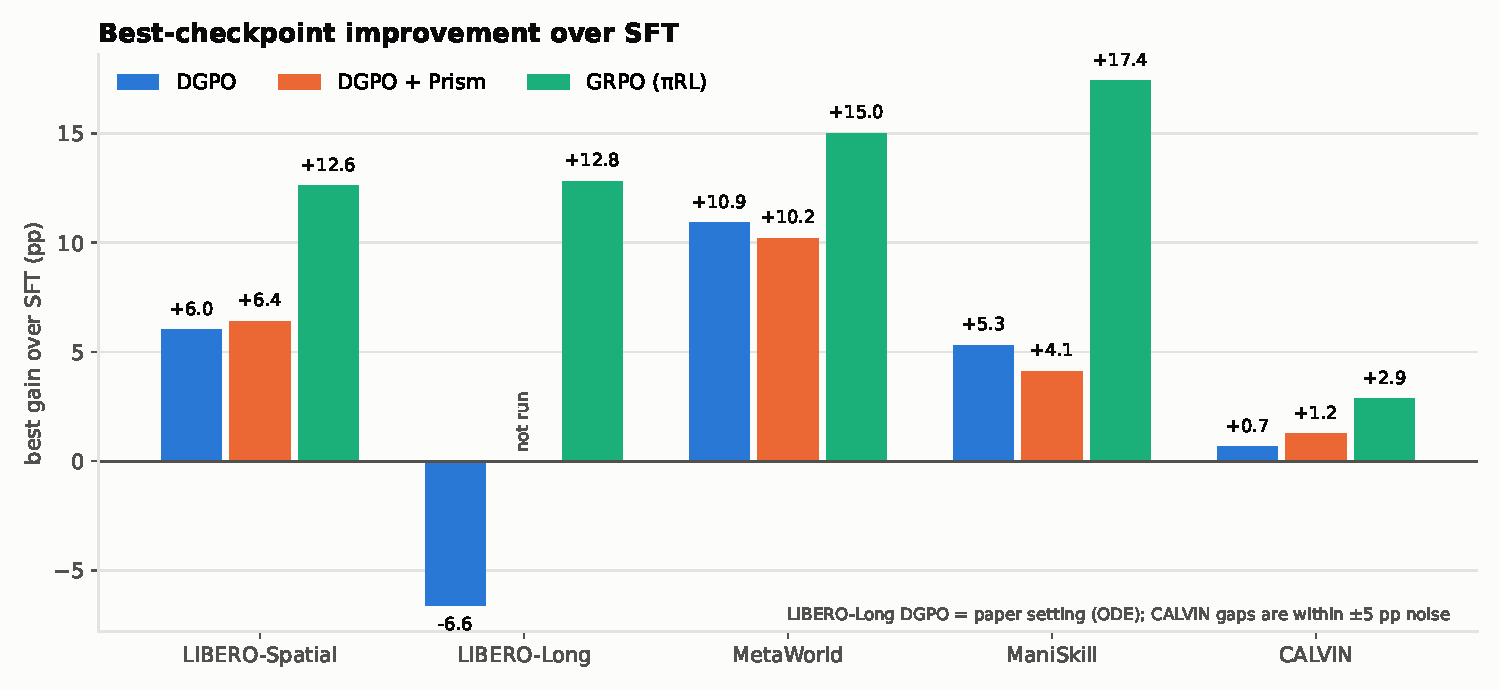
\includegraphics[width=0.9\linewidth]{fig1_summary_gain.pdf}\\
  \snote{DGPO $=$ SDE 0.3 on every denoise step, 2 updates per rollout, $\beta=10^4$ (LIBERO-Long: ODE only).}
\end{frame}

\begin{frame}{Learning curves}
  \centering
  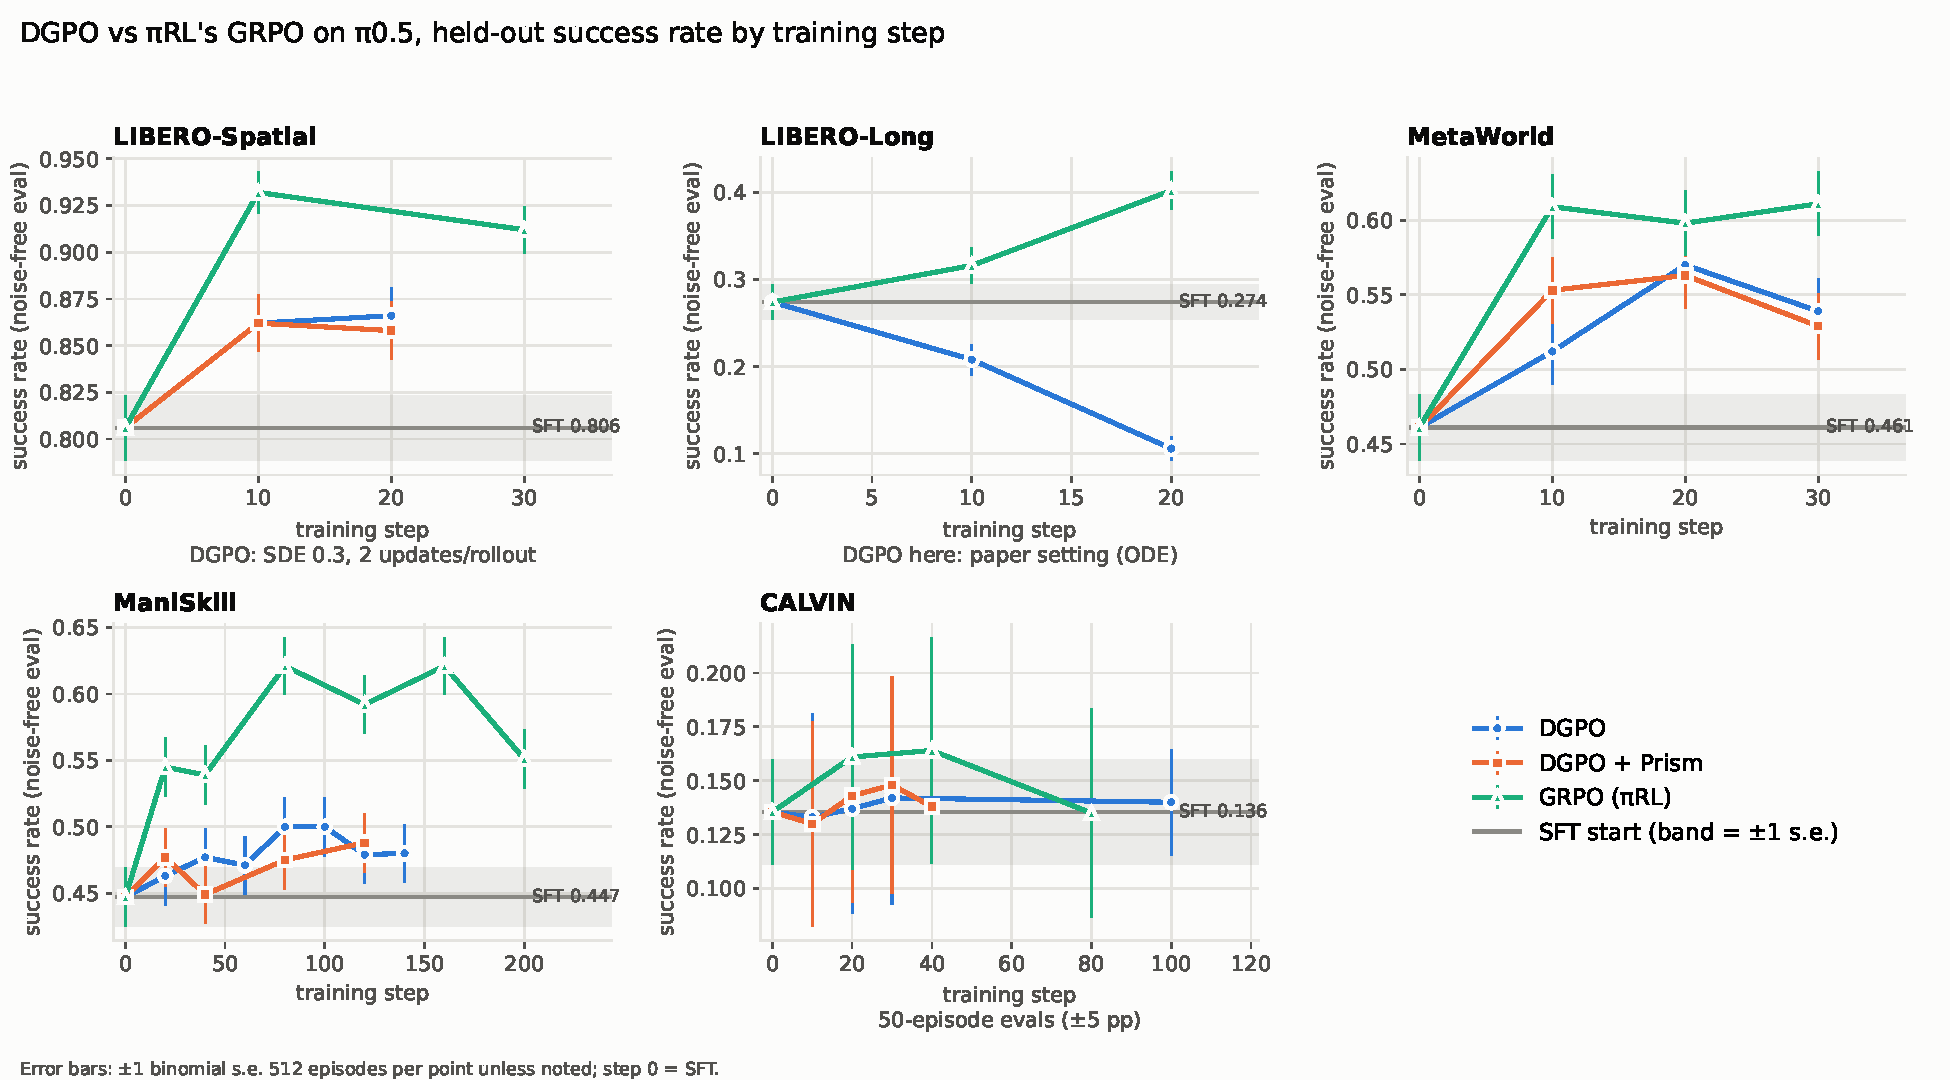
\includegraphics[width=0.93\linewidth]{fig2_learning_curves.pdf}
\end{frame}

\begin{frame}{Is it the noise? DGPO with GRPO's exact exploration noise}
  \centering
  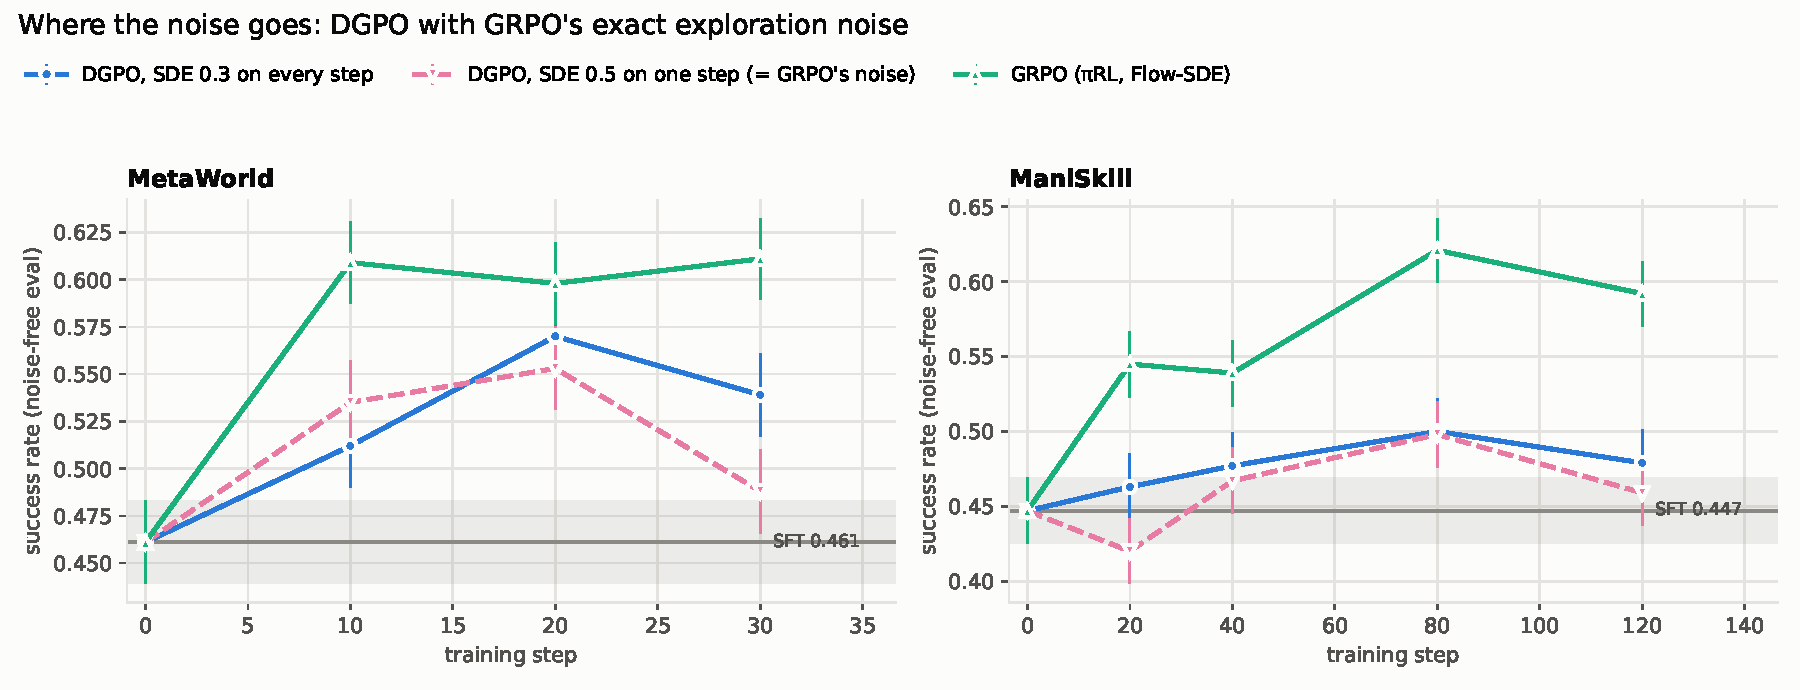
\includegraphics[width=0.95\linewidth]{fig6_noise_placement.pdf}\\
  \snote{New option \texttt{nft\_single\_noise\_step}: SDE noise 0.5 on one random denoise step, exactly as
  GRPO's rollouts. Step-1 training success matched GRPO's (MetaWorld 0.438 vs 0.422). The gap remains
  and the run is less stable, so \textbf{the gap is the update rule, not the noise}.}
\end{frame}

\begin{frame}{Is it tuning? One-knob sweep on MetaWorld}
  \centering
  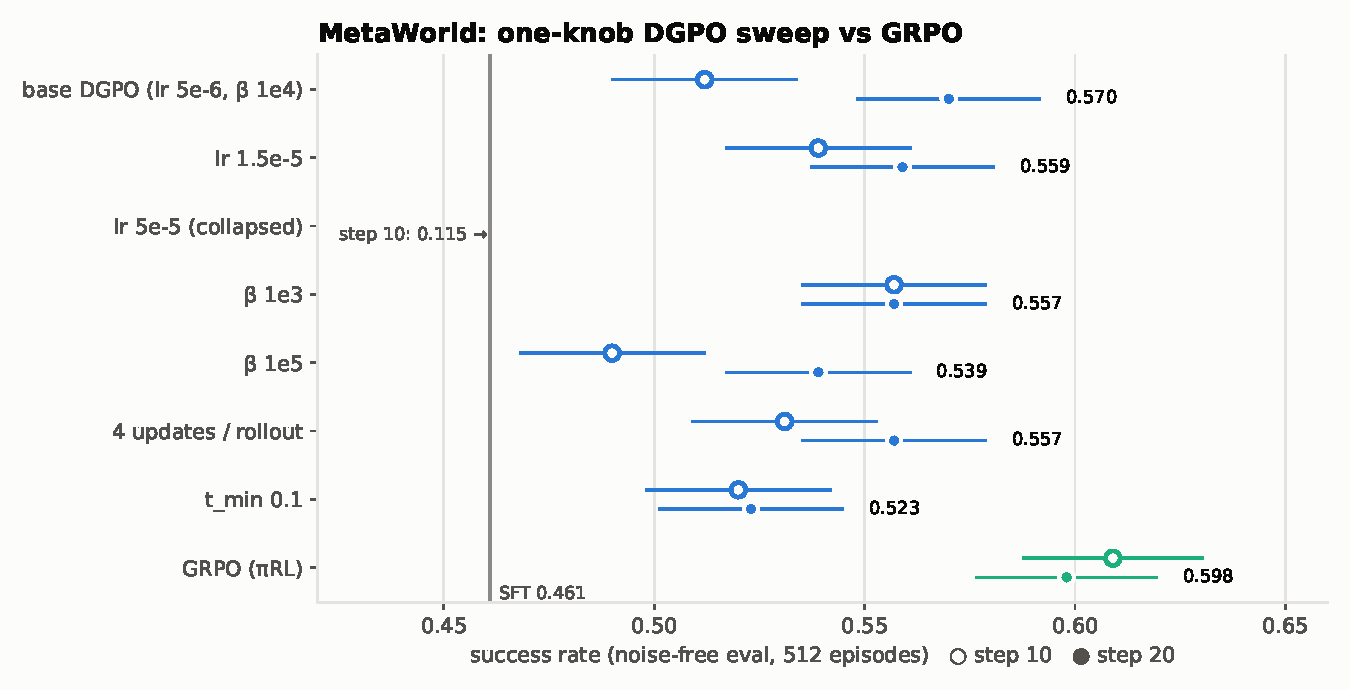
\includegraphics[width=0.74\linewidth]{fig4_metaworld_sweep.pdf}\\
  \snote{Nothing beats the base setting at step 20; every setting that learns plateaus at 0.52--0.57.}
\end{frame}

\begin{frame}{Stage 2: the Prism reward}
  \small
  \begin{itemize}
    \item $R=\text{success}+\lambda q$, $\lambda=0.5$, $q=\exp(-J/\mathrm{median}\,J)$ with $J$ the jerk of the
          executed continuous action dims (gripper excluded); RLOO advantage (zero-sum, so $Z$ still cancels);
          group filtering off.
    \item Result: no measurable gain anywhere (MetaWorld 0.563 vs 0.570, ManiSkill 0.488 vs 0.500,
          LIBERO-Spatial 0.862 vs 0.866, CALVIN within noise).
    \item Why: with SDE rollouts $\sim$90\% of groups are already mixed, so Prism's tie-breaking of
          same-outcome groups has little to act on (3--9\% of groups).
  \end{itemize}
\end{frame}

%==================================================================
\section{Discussion}
\begin{frame}{Why DGPO does not transfer to \pirl}
  \small
  \begin{enumerate}
    \item \textbf{The speed-up has nothing to remove here.} The 20--30$\times$ comes from
          (i) long SDE sampling and (ii) training along the whole denoising chain in Flow-GRPO.
          \pirl\ rollouts are simulator-bound (3--4 denoise steps), and its Flow-SDE already trains
          one random step. Measured: GRPO steps were 15--35\% \emph{faster} than DGPO's.
    \item \textbf{ODE rollouts carry no signal} once SFT is strong (previous section).
    \item \textbf{Early plateau everywhere}, even with the gate kept open ($\beta=10^3$):
          a DSM-difference preference over a 50--100-chunk trajectory with one binary reward is a
          weak, noisy signal compared with GRPO's per-transition likelihood ratio.
    \item \textbf{DGPO regresses onto the sampled $x_0$.} With large one-step noise the successful
          samples carry that noise, and the noise-free policy degrades (ManiSkill step 20: 0.420 $<$ SFT);
          GRPO optimises the noised transition's likelihood instead.
  \end{enumerate}
\end{frame}

\begin{frame}{Caveats}
  \small
  \begin{itemize}
    \item One seed per configuration (the gaps are large: 4--12 pp at 512 episodes, $\pm$2.2 pp s.e.).
    \item The trajectory-level extension is ours; DGPO is validated on single-sample generation.
    \item DGPO sweep was one knob at a time on MetaWorld; no LoRA, no combined tuning.
    \item CALVIN was scored with \texttt{success\_once}, not the paper's average chain length.
    \item Absolute numbers are below \pirl's (shorter training, 4 GPUs); we did not run PPO or \pizero.
    \item Training success (with exploration noise) is not a proxy for noise-free success:
          DGPO-1step led GRPO in training success at ManiSkill steps 10--12 and trailed it in eval.
  \end{itemize}
\end{frame}

\begin{frame}{Conclusions}
  \begin{itemize}
    \item Replacing \pirl's Flow-SDE GRPO with DGPO, as planned, \textbf{does not beat GRPO} on any of
          LIBERO, MetaWorld, ManiSkill or CALVIN.
    \item The paper's ODE setting degrades the policy; with SDE noise DGPO improves on SFT
          (+6 / +11 / +5 pp on LIBERO-Spatial / MetaWorld / ManiSkill) but GRPO does more
          (+13 / +15 / +17 pp).
    \item Not an implementation issue (matches the official gradient), not tuning (sweep), not the
          noise (identical rollouts): \textbf{the update rule}.
    \item Prism's reward adds nothing on top of DGPO in these benchmarks.
  \end{itemize}
  \vspace{0.5em}
  \textbf{Possible next steps:} DGPO + SDE on LIBERO-Long; \pizero; CALVIN with the paper's chain-length
  metric; Prism on GRPO for completeness (it is the Prism-GRPO paper's own setting).
\end{frame}

%==================================================================
\appendix
\begin{frame}{Backup: all held-out numbers (noise-free success)}
  \scriptsize
  \resizebox{\linewidth}{!}{%
  \begin{tabular}{@{}lllll@{}}
    \toprule
    Benchmark (SFT) & DGPO + SDE & DGPO + Prism & DGPO 1-step noise & GRPO \\
    \midrule
    LIBERO-Spatial (0.806) & .862 / .866 (s10/20) & .862 / .858 & -- & .932 / .912 (s10/30) \\
    LIBERO-Long (0.274) & ODE: .208 / .106 (s10/20) & -- & -- & .316 / .402 \\
    MetaWorld (0.461) & .512 / .570 / .539 (s10/20/30) & .553 / .563 / .529 & .535 / .553 / .488 & .609 / .598 / .611 \\
    ManiSkill (0.447) & .463/.477/.500/.479 (s20/40/80/120) & .477/.449/.475/.488 & .420/.467/.498/.459 & .545/.539/.621/.592 \\
    CALVIN (0.136) & .133/.137/.142 (s10/20/30), .140 (s100) & .130/.143/.148, .138 (s40) & -- & .161/.164/.135 (s20/40/80) \\
    \bottomrule
  \end{tabular}}\\[0.6em]
  {\scriptsize\textcolor{ink2}{512 episodes ($\pm$2.2 pp) except CALVIN: 50 episodes ($\pm$5 pp); CALVIN s100 / s40 and SFT: 200 episodes.
  Full log: \texttt{\textasciitilde/pirl-dgpo/README.md}.}}
\end{frame}

\end{document}
